%\documentclass[a4paper,12pt,pdftex,draft]{scrartcl}
\documentclass[a4paper,12pt,pdftex]{scrartcl}
%\documentclass[a4paper,12pt,pdftex,draft]{scrartcl}

\usepackage[american]{babel}
\usepackage[latin1]{inputenc}
%\usepackage{amsmath}
%\usepackage{amsfonts}


\usepackage{listings}
%\lstset{numbers=left, numberstyle=\tiny, numbersep=5pt}
\lstset{
  basicstyle=\ttfamily \scriptsize,
  showstringspaces=false
}
\lstset{xleftmargin=0cm}
\lstset{language=bash}
\lstset{frame=trBL}

\usepackage{graphicx}
%\usepackage{cmbright}   

\parindent0cm
\parskip2.5mm

\title{PIOSim MPIwrapper}
\author{Paul M�ller}

\begin{document}

\maketitle

\begin{abstract}
  The MPI wrapper is a static library that can be used to log MPI
  function calls which occur during the execution of a program. The
  log files are intended to be used by the PIOsimHD simulator project.

  This document describes the use, internal structure and extension
  possibilities of the MPI wrapper.
\end{abstract}

\tableofcontents

\section{Using the wrapper}

\subsection{Requirements}

The MPI wrapper project references the HDTraceWritingCLibrary
project. It must be built before building the MPI wrapper:
\begin{lstlisting}
cd PIOsimHD/HDTraceWritingCLibrary/
make
\end{lstlisting}

{\verb libglib} is also needed.

\subsection{Building the wrapper}

The MPI wrapper library can be built either for the mpich or openmpi
implementation of MPI. Due to differences between the implementations
you cannot use one version of the wrapper for both.

To build the library for mpich, call make:
\begin{lstlisting}
cd PIOsimHD/PIOsimHD-Maint/mpiwrapperNew/
make
\end{lstlisting}

To build the library for openmpi, set the environment variable
\lstinline|MPIIMP=openmpi|:
\begin{lstlisting}
cd PIOsimHD/PIOsimHD-Maint/mpiwrapperNew/
MPIIMP=openmpi make
\end{lstlisting}

\subsection{Building the tests}
The directory
\lstinline|PIOsimHD/PIOsimHD-Maint/mpiwrapperNew/test/HDTests|
contains a number of programs to test the functionality of the
wrapper. These tests can be build via
\begin{lstlisting}
cd PIOsimHD/PIOsimHD-Maint/mpiwrapperNew/
make hdtest
\end{lstlisting}

\subsection{Example: Producing a trace}
In this example, the PIOsim project tree is located in the home
folder, and the necessary libraries have been built as described
above. I am going to compile and trace the {\verb mpi-io-test } program
\cite{mpi-io-test}.
\begin{lstlisting}
cd $HOME
mkdir mpi-io-test
cd mpi-io-test/
wget http://mirror.anl.gov/pub/pvfs2/tests/mpi-io-test.c
mpicc -o mpi-io-test mpi-io-test.c \
 $HOME/PIOsimHD/PIOsimHD-Maint/mpiwrapperNew/libs/libHDTraceMPIWrapper.a \
 $HOME/PIOsimHD/HDTraceWritingCLibrary/lib/libhdTrace.a \
 `pkg-config --libs glib-2.0`
mpiexec -n 3 ./mpi-io-test
\end{lstlisting}  %$
Running the program will produce the following output

\begin{lstlisting}
# Using mpi-io calls.
nr_procs = 3, nr_iter = 1, blk_sz = 16777216, coll = 0
# total_size = 50331648
# Write: min_t = 1.177056, max_t = 1.613190, mean_t = 1.331647, var_t = 0.059641
# Read:  min_t = 0.448252, max_t = 0.544611, mean_t = 0.509273, var_t = 0.002816
Write bandwidth = 31.200076 Mbytes/sec
Read bandwidth = 92.417616 Mbytes/sec
D: [TRACER][node02.1.0] flushLog (hdTrace.c:955): flushing log length: 2172
D: [TRACER][node01.0.0] flushLog (hdTrace.c:955): flushing log length: 2130
D: [TRACER][node01.2.0] flushLog (hdTrace.c:955): flushing log length: 2172
\end{lstlisting}
This means everything went well and each of the three processes wrote
their own log files. The directory now contains three {\verb .xml } and
three {\verb .info } files. The latter need to be converted in order to
provide a format that is compatible with the simulator software and
other tools. The conversion is done via
\begin{lstlisting}
$HOME/PIOsimHD/PIOsimHD-Maint/mpiwrapperNew\
/scripts/project-description-merger.py \
  -o mpi-io-test.xml mpi-io-test_*.xml
\end{lstlisting} %$
The resulting four xml files can now be processed by other tools. Here
is an example of loading them into HDJumpshot:
\begin{figure}[h]
  \centering
  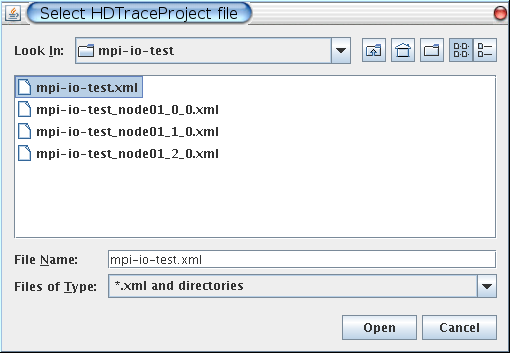
\includegraphics[scale=2]{img/jumpshot-open}
  \caption{Opening the project description file}
  \label{fig:jumpshot-open}
\end{figure}

\begin{figure}[h]
  \centering
  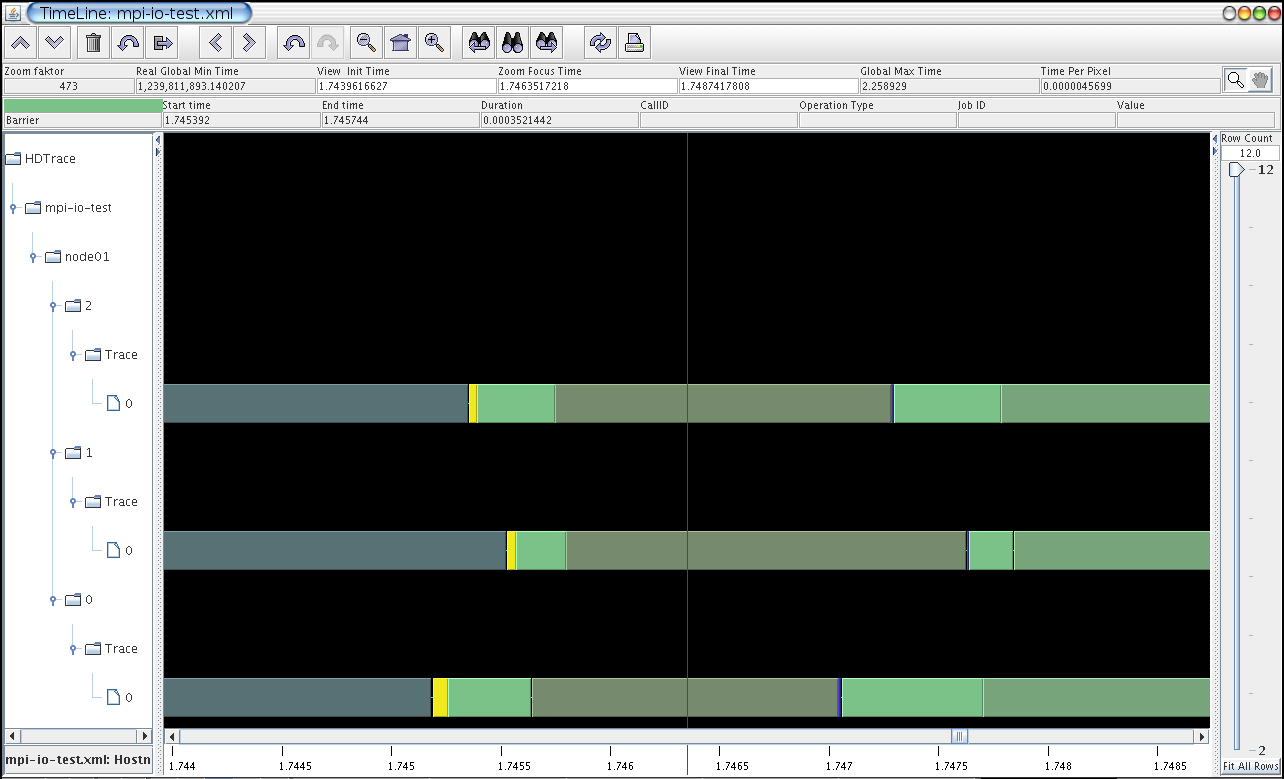
\includegraphics[scale=1]{img/jumpshot}
  \caption{mpi-io-test as displayed by Jumpshot}
  \label{fig:jumpshot}
\end{figure}

\section{Environment variables and command line options} 
\subsection{HDTraceMPIWrapper.a}
The behaviour of the tracing library can be adjusted by setting
certain environment variables before running a program. For example,
you can force flushing the write buffer on each write by setting
{\verb HDTRACE_FORCE_FLUSH }:
\begin{lstlisting}
HDTRACE_FORCE_FLUSH=1 ./mpi-io-test
\end{lstlisting}

The following variables are supported:

\subsubsection{HDTRACE\_FORCE\_FLUSH}
{\verb HDTRACE_FORCE_FLUSH=0 } means, the wrapper flushes the write
buffer on its own discretion, usually only when the buffer is full or
the file is closed. This is the default.

{\verb HDTRACE_FORCE_FLUSH=1 } causes the wrapper to flush the
write buffer on every write.


\subsubsection{HDTRACE\_NESTED}
This variable influences, whever nested function calls should be
traced. A nested call is a call to an MPI routine from within an MPI
routine.

{\verb HDTRACE_NESTED=0 } Only the outer function call is being logged.

{\verb HDTRACE_NESTED=1 } Nested calls up to a certain depth are
logged. The depth is determined by the constant {\verb
  HD_LOG_MAX_DEPTH }, defined in {\verb hdTrace.h }

\subsubsection{HDTRACE\_FILE\_INFO}
This variable determines, if the MPI\_Info structure that is given
to {\verb MPI_File_delete }, {\verb MPI_File_set_view }, {\verb
  MPI_File_set_info } or {\verb MPI_File_open } should be logged.   

{\verb HDTRACE_FILE_INFO=0 } The file information is not logged

{\verb HDTRACE_FILE_INFO=1 } The file information is logged

\subsubsection{HDTRACE\_ALL\_FUNCTIONS}
This variable determines, if ordinary functions should be logged. An
ordinary function is one that appears in {\verb
  include/interesting_funcs.h } but does not have any elements or
attributes other than start and end time being logged.

{\verb HDTRACE_ALL_FUNCTIONS=0 } ordinary functions are not logged.

{\verb HDTRACE_ALL_FUNCTIONS=1 } ordinary functions are logged. This
is the default.

\subsection{project-description-merger.py}

The project description merger creates a single xml file from the
collection of info files that have been written by the different MPI
processes. 

\subsubsection{Usage}
\begin{lstlisting}
project-description-merger.py -o <outfile.xml> [-d <description>] \
[--distribution-class=<class>] \
[--chunk-size=<size>] \
<log1>.info <log2>.info ... <logN>.info
\end{lstlisting}

\verb -o  \verb <outfile>  (required): The output file. The naming conventions for the
trace files are { \verb <program-name>_<hostname>_<rank>_<thread>.xml }. 

 It is advised to use { \verb <program-name>.xml } as output
 filename. This is expected by other PIOsim applications.

{ \verb -d  \verb <description> } (optional): The description of the
project. This can be anything. 

\section{Extending the wrapper}

The MPI wrapper redefines some of the functions that are provided by
the MPI library. These functions hide the original MPI functions when
the wrapper library (\verb libHDTraceMPIWrapper.a ) is linked to a
program. Thus, every call to an MPI function within the program is 
passed to a wrapper function. The wrapper function logs data about the
call to a log file (using the \verb HDTraceWritingCLibrary ) and
forwards the call to the corresponding PMPI function. mpich and
openmpi provide each function twice, once with the prefix {\verb MPI_ }
and once with the prefix \verb PMPI_  for exactly this purpose.

The wrapper functions have mostly the following shape:
\begin{lstlisting}
int MPI_<function>(<type 1> v1, ..., <type N> vN)
{
  int ret;

  hdT_StateStart(tracefile, "<function>");

  ret = PMPI_<function>( v1, ..., vN );

  <Eventually log elements using hdT_logElement(...)>

  <Eventually log attributes using hdT_logAttributes(...)>

  hdT_StateEnd(tracefile);
  return ret;
}
\end{lstlisting}

Because the wrapper functions have so much in common, they are
generated by a script instead of being written manually. The script
called is \verb scripts/create_sim-wrapper.py . It uses the
configuration file \verb scripts/wrapper_conf.py . The configuration
file is used to list the code parts that are inserted at certain
points into the wrapper function. 

The following example demonstrates,
what needs to be done to create a custom trace for an MPI function.

\subsection{Example: Tracing an MPI function}
Assume that you want to log every call to the \lstinline/MPI_Error_string/
function and the argument being passed to the function. 
\begin{enumerate}
\item Make sure that the function definition of {\lstinline[]/MPI_Error_string/} is
  listed in the file {\verb include/interesting_funcs.h }:
\begin{lstlisting}[title={include/interesting\_funcs.h}]
int MPI_Error_string(int, char *, int *);
\end{lstlisting}
\item Modify the \verb logAttributes  dictionary in 
{\verb scripts\wrapper_conf.py }. If you want to log the first
(\verb errorcode ) and the second (\verb errorstring ) arguments, you
have to enter the following
\begin{lstlisting}
logAttributes = {
  "Error_string" : ("code='%d' string='%s'",
                    "v1, v2"),
\end{lstlisting}
The key of the dictionary corresponds to the name of the function
without the \verb MPI_  prefix. The value is a tuple. The tuple's
first entry denotes the formatting of the attributes in printf-like
notation. It should have the form \verb key='value'  to produce a
valid xml file. The value should be enclosed in quotation marks.

The tuple's second entry is a comma separated list of parameters that
are used as arguments for the format string.

Building the wrapper will automatically produce the following wrapper
function:
\begin{lstlisting}
int MPI_Error_string(int v1,  char * v2,  int * v3){
  int ret;

  hdT_logStateStart(tracefile, "Error_string");

  ret = PMPI_Error_string( v1,  v2,  v3);

  hdT_logAttributes(tracefile, "code='%d' value='%s'", v1, v2);
  hdT_logStateEnd(tracefile);

  return ret;
}
\end{lstlisting}

\item
Now, you can compile and run the following test program. Make sure
to link the libraries \verb libHDTraceMPIWrapper.a , 
\verb libhdTrace  and \verb libglib-2.0  .
\begin{lstlisting}
#include <mpi.h>

char ecode[MPI_MAX_ERROR_STRING];
int len;

int main(int argc, char *argv[])
{
    MPI_Init(&argc, &argv);
    MPI_Error_string(0, ecode, &len);
    MPI_Finalize();
}
\end{lstlisting}

\end{enumerate}

\subsection{Logging an unspecified number of elements}

If you want to log an arbitrary number of items, using 
attributes won't do the trick. The answer is to log xml elements by
calling \verb hdT_logElement  before or after the call to the PMPI
function, depending on which parameters you want to log. This can be
accomplished by using the dictionaries \verb beforeMpi  and 
\verb afterMpi . An example is the logging of {\verb Alltoallv }
that has to write the size of each block that is sent to the other ranks.
This is the entry in the dictionary \verb afterMpi . It maps the
function's basename to a code snippet that is inserted after the 
\verb PMPI_Alltoallv  call.
\begin{lstlisting}
afterMpi = {
[...]
"Alltoallv" : """
  {
    int size, i;
    MPI_Comm_size(v9, &size);
    for(i = 0; i < size; ++i)
    {
      hdT_LogElement(tracefile, "Send", "rank='%d' size='%lld' count='%d' type='%d'",
                   getWorldRank(i, v9), getTypeSize(v2[i], v4), v2[i], getTypeId(v4));
    }
  }
""",
\end{lstlisting}
As you can see, the functions's arguments \verb v1 ...\verb v9  are
passed to \verb hdT_LogElement  which formats its arguments similar to
printf.

All functions that are defined in or included from 
\verb HDTraceMPIWrapper.src.c  can be used.

\subsection{Logging MPI\_File, MPI\_Comm, MPI\_Datatype and MPI\_Request datatypes}
It is necessary to log certain MPI structures such as \verb MPI_File , 
\verb MPI_Comm ,
\verb MPI_Datatype and
\verb MPI_Request . The file \verb hash_tables.c  provides an
interface to log these functions. When you need to log an MPI
datatype, you can call \verb getTypeId(datatype)  which will return an
integer ID that can be logged. The function
 \verb getTypeId()  accesses an internal hash map and associates a new
 ID with 
\verb datatype . If the datatype has already been accessed, the
previously associated ID is returned. 

\bibliography{references}
\bibliographystyle{alpha}

\end{document}
